\section{Scenarios}
\begin{frame}{Scenarios}
rootJS is used by applications to access the ROOT framework\\
\pause $\Rightarrow $ our users are those applications
\end{frame}

\subsection{Event Viewer}
\begin{frame}{Event Viewer}
 \pause   Event Viewers provide visualisation of experimental data
  \begin{itemize}
    \pause \item useful for quick eyescan of data
    \pause \item quickly check if data is recorded properly
  \end{itemize}
  \pause
  \medskip
   Conventional ROOT Event Viewer
  \begin{itemize}
  \pause \item standalone ROOT application
   \pause \item requires ROOT on machine
   \pause \item requires ROOT's dependencies
   \pause \item requires access to data source
   \end{itemize}
   \pause $\Rightarrow $ very limited portability and harsh requirements for client system
\end{frame}

\begin{frame}{Event Viewer}
 Event Viewers provide visualisation of experimental data
  \begin{itemize}
   \item useful for quick eyescan of data
   \item quickly check if data is recorded properly
  \end{itemize}
   \medskip
   Client/Server based Web Event Viewer based on nodeJS
  \begin{itemize}
  \pause \item server runs ROOT and its dependencies
   \pause \item client only needs modern web browser
   \pause \item no access to critical data sources required
   \pause \item no heavy work load on client system
   \end{itemize}
   \pause $\Rightarrow $ great portability and ease of use as client can be almost any device
\end{frame}


\begin{frame}{Event Viewer}
  \begin{figure}[htb]
      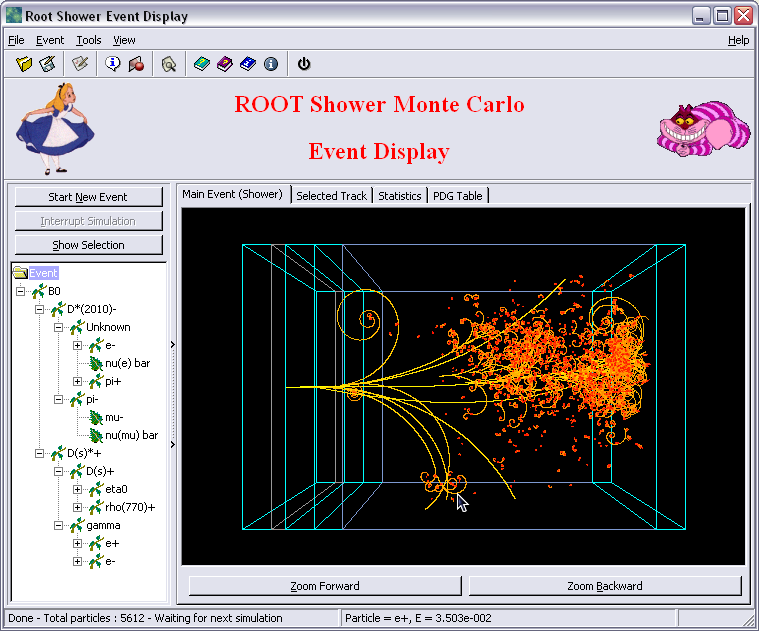
\includegraphics[width=0.97\linewidth, keepaspectratio]{./resources/shower_event_viewer.png}
      \nocite{cern:root:eventviewer}
   \end{figure}
\end{frame}
